\chapter{Решение уравнений с немонотонным оператором}
Монотонность оператора $A$ исходного уравнения --- очень сильное требование, которое не выполняется во многих важных прикладных задачах, например, в задачах гравиметрии и магнитометрии. В данной главе показано, что в конечномерном случае есть возможность ослабить условие монотонности и обосновать сходимость итераций методов РМН, ММО, МНС, ММН.
В первом параграфе представлены доказательства сходимости метода Ньютона с регуляризацией, во втором параграфе доказаны теоремы сходимости для нелинейных аналогов $\alpha$-процессов, в третьем параграфе представлены следствия для модифицированных аналогов $\alpha$-процессов и оценка невязки двухэтапного метода, в четвертом приведены результаты численного моделирования.

\newpage
\section{Метод Ньютона}
Рассматривается конечномерный случай, когда оператор $A\colon R^n \to R^n$, для которого матрица $A'(u)$ в некоторой окрестности решения имеет спектр, состоящий из различных неотрицательных собственных значений.
Приведем лемму (В.В. Васин, \cite{VasSkur2017}).
\begin{lemma}\label{lemVas}
	Пусть $n\times n$ матрица $A'(u)$ не имеет кратных собственных значений $\lambda _i$ и числа $\lambda _i$ ($i=1,2,..n$) различны и неотрицательны. Тогда при $\bar\alpha>0$ матрица имеет представление $A'(u)+\bar\alpha I =S(u)\Lambda S^{-1}(u)$ и справедлива оценка
	\begin{equation}\label{est4.1}
	\|(A'(u)+\bar\alpha I)^{-1}\|\le \frac{\mu (S(u))}{\bar\alpha+\lambda_{min}} \le \frac{\mu(S(u))}{\bar\alpha},
	\end{equation}
	где столбцы матрицы $S(u)$ составлены из собственных векторов матрицы $A'(u)+\bar\alpha I$, $\Lambda$ --- диагональная матрица, ее элементы --- собственные значения матрицы $A'(u)+\bar\alpha I$, $\mu(S(u))=\|S(u)\|\|S^{-1}(u)\|$.
\end{lemma}
Обратимся к регуляризованному методу Ньютона, для которого была доказана теорема $\ref{teo2.3}$ о сходимости итераций и оценке погрешности для монотонного оператора. Рассмотрим теперь вариант этой теоремы, когда оператор $A\colon R^n \to R^n$, матрица производной $A'(u)$ которого имеет неотрицательный спектр, удовлетворяющий условиям леммы $\ref{lemVas}$, причем функция $\mu(S(u))$ при фиксированном $\alpha$ равномерно ограничена по $u$ в шаре $S(r, u_\alpha)$, т.е.
\begin{equation}\label{cond4.3}
\sup\{\mu(S(u)): u\in S(r, u_\alpha)\}\le\bar S <\infty .
\end{equation}
\begin{theorem}\label{teo4.1}
	Пусть выполнены условия $\eqref{cond4.3}$, $\eqref{cond1.1}$--$\eqref{cond1.3}$, $A'(u^0)$ --- симметричная матрица, и для параметров $\alpha$, $\bar{\alpha}$, $r$ справедливы соотношения: $0<\alpha\le\bar\alpha$, $\bar\alpha\ge 4N_0$, $r\le\alpha/8N_2\bar S$, $\|u_\alpha-u^0\|\le r$.
	Тогда для метода $\eqref{equ_rmn}$ справедливо заключение теоремы $\ref{teo2.3}$, где соотношения $\eqref{ineq2.12}$, $\eqref{eq2.13}$ для $\gamma$ и выражение для $q$ в $\eqref{est2.16}$ соответственно принимает вид
	$$\gamma < \frac{\alpha\bar\alpha}{2(N_1+\alpha)^2\bar S^2}, \quad \gamma _{opt}=\frac{\alpha\bar\alpha}{4(N_1+\alpha)^2\bar S^2}, \quad q=\sqrt{1-\frac{\alpha ^2}{16(N_1+\alpha)^2\bar S^2}}$$
\end{theorem}
\begin{proof} С учетом оценки $\eqref{est4.1}$, доказательство с несущественными поправками проводится по схеме доказательтства теоремы $\ref{teo2.3}$.
\end{proof}

{\remark При доказательстве теоремы вместо условия  $\eqref{cond4.3}$ достаточно требовать ограниченность величины $\sup\{\mu(S(u^k)): u^k \in S_r(u_\alpha)\}$, где $u^k$ --- итерационные точки метода. Причем, при регулярном правиле останова итераций $k(\delta)$, супремум берется по конечному набору номеров $k\le k(\delta)$, что автоматически влечет ограниченность супремума и выполнение оценки вида $\eqref{est2.16}$ при этих значениях $k$. Кроме того, для модифицированного метода Ньютона, в котором производная $A'(u^0)$ вычисляется в фиксированной точке $u^0$, величина $\mu(S(u^0))=\|S(u^0)\|\|S^{-1}(u^0)\|=\bar S<\infty$.}

\newpage
\section{Нелинейные аналоги альфа-процессов}
При тех же условиях на оператор, что и для метода Ньютона в параграфе 2.1, исследуем процессы $\eqref{equ_alphaproc}$.
\begin{theorem}\label{teo4.2}
	Пусть выполнены условия $\eqref{cond1.1}$--$\eqref{cond1.3}$. Пусть при $u \in S_r(u_\alpha)$ матрица $A'(u)$ имеет спектр, состоящий из неотрицательных различных собственных значений, $A'(u^0)$ --- симметричная неотрицательно определенная матрица. Пусть параметры $\alpha$, $\bar{\alpha}$, $r$ удовлетворяют условиям: 
	\begin{equation}\label{cond4.4}
	MMO:\qquad 0<\alpha\le\bar\alpha, \quad r\le\alpha /6\bar SN_2, \quad \bar\alpha \ge N_0
	\end{equation}
	\begin{equation}\label{cond4.5}
	MHC:\qquad 0<\alpha\le\bar\alpha, \quad r\le\alpha /3N_2,
	\end{equation}
	\begin{equation}\label{cond4.6}
	MMH:\qquad 0<\alpha\le\bar\alpha, \quad r\le\alpha /6N_2.
	\end{equation}
	Тогда справедливы соотношения  $\eqref{ineq3.4}$, где
	\begin{equation}\label{eq4.7}
	\mu _{-1}=\frac{8\bar S^2(N_1+\alpha)^2}{\alpha\bar\alpha}, \quad \mu _0=\frac{18(N_1+\alpha)^2(N_1+\bar\alpha)}{\alpha\bar\alpha ^2}, \quad \mu _1=\frac{18(N_1+\alpha)^2(N_1+\bar\alpha)^4}{\alpha\bar\alpha ^5}
	\end{equation}
\end{theorem}
\begin{proof} При $\varkappa=-1$ и тех же обозначениях, которые были приняты в разделе 3, получим (нижний индекс (-1) соответствует методу $\eqref{equ_alphaproc}$ при $\varkappa=-1$)
$$\langle F_{-1}(u), u-u_\alpha\rangle=\beta _{-1}(u)[\langle A(u)-A(u_\alpha), u-u_\alpha\rangle+\alpha\|u-u_\alpha\|^2].$$
Оценим каждое из слагаемых в правой части равенства с учетом условий $\eqref{cond4.4}$, используя формулу Лагранжа:
$$\langle A(u)-A(u_\alpha), u-u_\alpha\rangle+\alpha\|u-u_\alpha\|^2=\alpha\|u-u_\alpha\|^2$$ $$+\langle \int\limits_0^1 (A'(u_\alpha+\theta(u-u_\alpha))-A'(u^0))(u-u_\alpha)d\theta, u-u_\alpha\rangle+\langle A'(u^0)(u-u_\alpha), u-u_\alpha\rangle$$ $$\ge \alpha\|u-u_\alpha\|^2-\frac{N_2(\|u^0-u_\alpha\|+\|u-u^0\|)^2}{2}\|u-u_\alpha\|^2$$
\begin{equation}\label {est4.8}
\ge\left ( \alpha-\frac{3N_2 r}{2}\right )\|u-u_\alpha\|^2\ge\frac{3\alpha}{4}\|u-u_\alpha\|^2
\end{equation}
$$\beta _{-1}(u)=\frac{\langle (A'(u)+\bar\alpha I)^{-1}S_\alpha(u), S_\alpha(u)\rangle}{\|S_\alpha(u)\|^2}=\frac{\langle (A'(u^0)+\bar\alpha I)^{-1}S_\alpha(u), S_\alpha(u)\rangle}{\|S_\alpha(u)\|^2}$$ $$+\frac{\langle (B^{-1}(u)-B^{-1}(u^0))S_\alpha(u), S_\alpha(u)\rangle}{\|S_\alpha(u)\|^2}\ge\frac{1}{N_0+\bar\alpha}-\frac{\bar S N_2\|u-u^0\|}{\bar\alpha^2}$$
\begin{equation}\label{est4.9}
\ge\frac{1}{N_0+\bar\alpha}-\frac{2\bar S N_2 r}{\bar\alpha^2}\ge\frac{1}{6\bar\alpha},
\end{equation}
где учтены условия $\eqref{cond4.4}$ и соотношение $\|u-u^0\|\le\|u-u_\alpha\|+\|u_\alpha-u^0\|\le 2r$.

Кроме того, справедлива оценка
$$\|F_{-1}(u)\|^2\le(\beta_{-1}(u))^2\|A(u)-A(u_\alpha)+\alpha(u-u_\alpha)\|^2$$
\begin{equation}\label{est4.10}
\le\|B^{-1}(u)\|^2(N_1+\alpha)^2\|u-u_\alpha\|^2\le\frac{\bar S^2(N_1+\alpha)^2}{\bar\alpha^2}\|u-u_\alpha\|^2
\end{equation}
Объединяя $\eqref{est4.8}$--$\eqref{est4.10}$, получаем, что в соотношении $\eqref{ineq3.4}$, $\mu_{-1}$ выражается величиной из $\eqref{eq4.7}$

Исследуем теперь МНС, т.е. процесс $\eqref{equ_alphaproc}$ при $\varkappa=0$. Аналогично предыдущему методу устанавливаем, что
\begin{equation}\label{est4.11}
\langle A(u)-A(u_\alpha), u-u_\alpha\rangle+\alpha\|u-u_\alpha\|^2\ge\left(\alpha-\frac{3N_2 r}{2}\right)\|u-u_\alpha\|^2
\end{equation}
Кроме того,
$$\beta_0(u)=\frac{\|S_\alpha(u)\|^2}{\langle B(u)S_\alpha(u), S_\alpha(u)\rangle}\ge\frac{1}{\|B(u)\|}\ge\frac{1}{\|A'(u)+\bar\alpha I\|}\ge\frac{1}{N_1+\bar\alpha}.$$
Объединяя последнее соотношение с $\eqref{est4.11}$, получаем оценку снизу
\begin{equation}\label{est4.12}
\langle F_0(u), u-u_\alpha\rangle\ge\frac{1}{N_1+\bar\alpha}\left (\alpha -\frac{3N_2 r}{2}\right )\|u-u_\alpha\|^2.
\end{equation}
Аналог оценки $\eqref{est4.10}$ для $F_0(u)$ следует из неравенств ниже:
\begin{equation}\label{est4.13}
\|F_0(u)\|\le\beta_0(u)(\|A(u)-A(u_\alpha)\|+\alpha\|u-u_\alpha\|)\le\beta_0(u)(N_1+\alpha)\|u-u_\alpha\|,
\end{equation}
$$\beta_0(u)=\frac{\|S_\alpha(u)\|^2}{\bar\alpha\|S_\alpha(u)\|^2+\langle A'(u^0)S_\alpha(u), S_\alpha(u)\rangle+\langle (A'(u)-A'(u^0))S_\alpha(u), S_\alpha(u)\rangle}$$
$$\le \frac{\|S_\alpha(u)\|^2}{\bar\alpha\|S_\alpha(u)\|^2-|\langle (A'(u)-A'(u^0))S_\alpha(u), S_\alpha(u)\rangle|}$$
\begin{equation}\label{est4.14}
\le\frac{1}{\bar\alpha -N_2\|u-u^0\|}\le\frac{1}{\bar\alpha -2N_2 r}
\end{equation}
Из $\eqref{est4.12}$-$\eqref{est4.14}$ при значениях параметров из $\eqref{cond4.5}$ получаем значения $\mu_0$ в $\eqref{eq4.7}$.

Наконец рассмотрим процесс $\eqref{equ_mmn}$ при $\varkappa=1$. Как и в предыдущем методе, при оценке снизу величины $\langle F_1(u), u-u_\alpha\rangle$, справедливо соотношение $\eqref{est4.11}$. Для параметра $\beta_1(u)$ получаем
$$\beta_1(u)=\frac{\langle B(u)S_\alpha(u), S_\alpha(u)\rangle}{\|B(u)S_\alpha(u)\|^2}$$$$\ge\frac{\langle A'(u^0)S_\alpha(u), S_\alpha(u)\rangle+\bar\alpha\langle S_\alpha(u), S_\alpha(u)\rangle-\|A'(u)-A'(u^0)\|\|S_\alpha(u)\|^2}{(N_1+\bar\alpha)^2\|S_\alpha(u)\|^2}$$$$\ge\frac{\bar\alpha -N_2\|u-u^0\|}{(N_1+\bar\alpha)^2}\ge\frac{\bar\alpha -2N_2 r}{(N_1+\bar\alpha)^2},$$
что при условиях на параметры $\eqref{cond4.6}$, дает оценку
\begin{equation}\label{est4.15}
\langle F_1(u), u-u_\alpha\rangle\ge\left (\alpha -\frac{3N_2 r}{2}\right )\frac{\bar\alpha - 2N_2 r}{(N_1+\bar\alpha)^2}\|u-u_\alpha\|^2\ge\frac{\alpha\bar\alpha}{2(N_1+\bar\alpha)^2}\|u-u_\alpha\|^2.
\end{equation}

Поскольку
$$\|F_1(u)\|\le\beta_1(u)(\|A(u)-A(u_\alpha)\|+\alpha\|u-u_\alpha\|)\le \beta_1(u)(N_1+\alpha)\|u-u_\alpha\|,$$ $$\|\beta_1(u)\|\le\frac{(N_1+\bar\alpha)\|S_\alpha(u)\|^2}{\|A'(u)S_\alpha(u)\|^2+2\bar\alpha\langle A'(u)S_\alpha(u), S_\alpha(u)\rangle+\bar\alpha^2\|S_\alpha(u)\|^2}$$ $$\le\frac{(N_1+\bar\alpha)\|S_\alpha(u)\|^2}{2\bar\alpha\langle A'(u^0)S_\alpha(u), S_\alpha(u)\rangle-2\bar\alpha|\langle (A'(u)-A'(u^0))S_\alpha(u), S_\alpha(u)\rangle|+\bar\alpha^2\|S_\alpha(u)\|^2}$$$$
\le\frac{(N_1+\bar\alpha)}{\bar\alpha^2-2\bar\alpha N_2\|u-u^0\|}\le\frac{N_1+\bar\alpha}{\bar\alpha(\bar\alpha - 4N_2 r)}\le\frac{3(N_1+\bar\alpha)}{\bar\alpha^2}.$$
Окончательно получаем для $\|F_1(u)\|^2$ оценку сверху
\begin{equation}\label{est4.16}
\|F_1(u)\|^2\le\frac{3^2(N_1+\alpha)^2(N_1+\bar\alpha)^2}{\bar\alpha^4}\|u-u_\alpha\|^2.
\end{equation}
Объединяя соотношения $\eqref{est4.15}$ и $\eqref{est4.16}$, и условия $\eqref{cond4.6}$, получаем значение $\mu_1$, представленное в $\eqref{eq4.7}$.
\end{proof}
\begin{theorem}\label{teo4.3}
	Пусть выполнены условия теоремы $\ref{teo4.1}$. Тогда при $\gamma<2/\mu _\varkappa$, $\varkappa=-1,0,1$, где значения $\mu _\varkappa$ определяются соотношениями $\eqref{eq4.7}$, последовательности ${u^k}$, порождаемые процессами $\eqref{equ_alphaproc}$, $\eqref{equ_mmn}$ при $\varkappa=-1,0,1$, сходятся к $u_\alpha$, т.е. $$\lim_{k\to\infty}\|u^k-u_\alpha\|=0,$$ а при $
	\gamma{_\varkappa^{opt}}=\frac{1}{\mu_\varkappa}$
	справедлива оценка $\|u^{k+1}-u_\alpha\|\le q{_\varkappa^k}r,$ где
	$$
	q_{-1}=\sqrt{1-\frac{\alpha^2}{64\bar S^2(N_1+\alpha)^2}}, \quad q_0=\sqrt{1-\frac{\alpha^2\bar\alpha^2}{36(N_1+\alpha)^2(N_1+\bar\alpha)^2}},$$
	\begin{equation}\label{eq4.17}
	q_1=\sqrt{1-\frac{\alpha^2\bar\alpha^6}{36(N_1+\alpha)^2(N_1+\bar\alpha)^6}}.
	\end{equation}
\end{theorem}
\begin{proof} Подставляя в соотношение $\eqref{ineq2.20}$ вместо $F(u^k)$ последовательность $F_\varkappa(u^k)$ ($\varkappa=-1,0,1$) и, используя оценки $\eqref{est4.8}$, $\eqref{est4.9}$ ($\varkappa=-1$), $\eqref{est4.9}$, $\eqref{est4.10}$ ($\varkappa=0$), $\eqref{est4.11}$, $\eqref{est4.12}$ ($\varkappa=1$), а также условия на параметры $\eqref{cond4.4}$--$\eqref{cond4.6}$, получаем, после минимизации по $\gamma$, значения для $q_\varkappa$, представленные в $\eqref{eq4.17}$. При выполнении условия $\gamma<2/\mu_\varkappa$, выражение в круглых скобках в правой части неравенства $\eqref{ineq2.20}$ принимает значение, которое меньше единицы, что влечет сходимость итераций для всех трех методов.
\end{proof}

{\remark Предложенный подход к получению оценок скорости сходимости итерационных процессов полностью переносится на случай, когда спектр матрицы $A'(u^k)$, состоящий из различных вещественных значений, содержит набор малых по абсолютной величине отрицательных собственных значений.} 

Пусть $\lambda _1$ --- отрицательное собственное значение с наименьшим модулем $|\lambda_1|$ и $\bar\alpha -|\lambda _1|=\bar\alpha _1<\alpha^*$. Тогда оценка $\eqref{est4.1}$ трансформируется в неравенство
\begin{equation}\label{ineq4.16}
\|(A'(u^k)+\bar\alpha I)^{-1}\|\le\frac{\mu(S(u^k))}{\bar\alpha^*}\le\frac{\bar S}{\bar\alpha^*}
\end{equation}
Все утверждения, т.е. теоремы $(\ref{teo4.1})$--$(\ref{teo4.3})$ остаются справедливыми при замене $\bar\alpha$ на $\bar\alpha^*$ во всех оценках, где используется $\eqref{ineq4.16}$.

{\remark Если рассматривать модифицированные варианты методов $\eqref{equ_rmn}$--$\eqref{equ_alphaproc}$, когда вместо $A'(u^k)$ в операторе шага используется $A'(u^0)$ в процессе итераций, то при условиях на оператор, принятых в данном разделе, для получения аналогичных результатов о сходимости и оценке погрешности наряду с неотрицательностью спектра достаточно требовать симметричность матрицы $A'(u^0)$ \cite{VasAkiMin2013, Vasin2014, Vasin2016}. Заметим, что при исследовании основных методов $\eqref{equ_rmn}$--$\eqref{equ_alphaproc}$ существование симметричной матрицы для некоторого элемента $u^0$ предполагается.}

\newpage
\section{Модифицированные варианты регуляризованных методов на основе нелинейных налогов альфа-процессов}
Рассматривается случай, когда производная оператора $A'(u)$ вычисляется в начальной точке итерационных процессов $u^0$. Тогда формулы итерационных процессов $\eqref{equ_alphaproc}$ принимают вид:
%модифицированный метод минимальной ошибки (МММО)
%\begin{equation}\label{m3o}
%u^{k+1}=u^k-\gamma\frac{\langle (A'(u^0)+\bar{\alpha}I)^{-1}S_\alpha(u^k),S_\alpha(u^k)>}{\|S_\alpha(u^k)\|^2}S_\alpha(u^k)\equiv T(u^k),
%\end{equation}
%модифицированный метод наискорейшего спуска (ММНС)
%\begin{equation}\label{m2ns}
%u^{k+1}=u^k-\gamma\frac{\|S_\alpha(u^k)\|^2}{\langle (A'(u^0)+\bar{\alpha}I)S_\alpha(u^k),S_\alpha(u^k)>}S_\alpha(u^k),
%\end{equation}
%модифицированный метод минимальных невязок (МММН)
%\begin{equation}\label{m3n}
%u^{k+1}=u^k-\gamma\frac{\langle (A'(u^0)+\bar{\alpha}I)S_\alpha(u^k),S_\alpha(u^k)>}{\|(A'(u^0)+\bar{\alpha}I)S_\alpha(u^k)\|^2}S_\alpha(u^k).
%\end{equation}
%Все три метода можно кратко записать в виде
\begin{equation}\label{modalphaproc}
u^{k+1}=u^k-\gamma\frac{\langle (A'(u^0)+\bar\alpha I)^{\varkappa}S_\alpha(u^k), S_\alpha(u^k)\rangle}{\langle (A'(u^0)+\bar\alpha I)^{\varkappa+1}S_\alpha(u^k), S_\alpha(u^k)\rangle}S_\alpha(u^k)\equiv T(u^k),
\end{equation}
где при $\varkappa=-1$ итерационный процесс представляет собой модифицированный ММО, при $\varkappa=0$ --- модифицированный МНС и при $\varkappa=1$ --- модифицированный ММН.

Справедлива следующая теорема.
\begin{theorem}\label{teomodalpnomonot}
	Пусть выполнены условия $\eqref{cond1.1}$--$\eqref{cond1.3}$,
$A'(u^0)$ --- самосопряженный оператор, спектр которого состоит из неотрицательных различных собственных значений, параметры $\alpha$, $\bar{\alpha}$, $r$ удовлетворяют условиям:
	\begin{equation}\label{cond2.4}
	0\le\alpha\le\bar{\alpha}, \quad r=\alpha/6N_2, \quad \bar{\alpha}\ge N_0.
	\end{equation}
	
	Тогда для оператора
	$$F_\varkappa^0(u)=\beta_{\varkappa}^0(u)S_\alpha(u),$$ где 
	$$\beta_{\varkappa}^0(u)=\frac{\langle (A'(u^0)+\bar\alpha I)^{\varkappa}S_\alpha(u), S_\alpha(u)\rangle}{\langle (A'(u^0)+\bar\alpha I)^{\varkappa+1}S_\alpha(u), S_\alpha(u)\rangle},$$ имеет место неравенство
	$$\|F_\varkappa^0(u)\|^2\le\frac{8(N_1+\alpha)^2}{3\alpha\bar{\alpha}}\langle F_\varkappa^0(u), u-u_\alpha\rangle,$$
	где $\varkappa=-1, 0, 1,$ для модифицированных вариантов ММО, МНС и ММН соответственно.
\end{theorem} 
\begin{proof} Получим оценку снизу скалярного произведения $\langle F_{-1}^0(u),u-u_\alpha\rangle$ для модифицированного ММО.
$$\langle F_{-1}^0(u),u-u_\alpha\rangle=\langle F_{-1}^0(u)-F_{-1}^0(u_\alpha),u-u_\alpha\rangle=\beta_{-1}^0(u)[\langle A(u)-A(u_\alpha),u-u_\alpha\rangle$$ $$+\alpha\|u-u_\alpha\|^2].$$
Оценим снизу $\langle A(u)-A(u_\alpha),u-u_\alpha\rangle$, используя формулу Лагранжа: $$\langle A(u)-A(u_\alpha),u-u_\alpha\rangle=\langle\int_{0}^{1}[A'(u_\alpha+\theta(u-u_\alpha))-A'(u^0)](u-u_\alpha)d\theta, u-u_\alpha\rangle$$ $$+\langle A'(u^0)(u-u_\alpha), u-u_\alpha\rangle\ge-N_2\int_{0}^{1}\|u_\alpha-u^0+\theta(u-u_\alpha)\|\cdot\|u-u_\alpha\|^2d\theta$$ $$=-N_2\|u-u_\alpha\|^2\int_{0}^{1}\|u_\alpha-u^0+\theta u-\theta u_\alpha\pm\theta u^0\|d\theta=-N_2\|u-u_\alpha\|^2$$
$$\times\int_{0}^{1}\|(1-\theta)(u_\alpha-u^0)+\theta(u-u_\alpha)\|d\theta\ge-N_2\|u-u_\alpha\|^2\Big[\int_{0}^{1}(1-\theta)d\theta\cdot\|u^0-u_\alpha\|$$$$+\int_{0}^{1}\theta d\theta\|u-u_\alpha\|^2\Big]=-N_2\|u-u_\alpha\|^2\Big[\frac{\|u_\alpha-u^0\|}{2}+\frac{\|u_\alpha-u^0+u^0-u\|}{2}\Big]$$
\begin{equation}\label{estmodif2.5}
\ge-\frac{3N_2r}{2}\|u-u_\alpha\|^2,
\end{equation}
где $r=\|u_\alpha-u^0\|,\quad \|u-u^0\|\le 2r$.

Получим оценку снизу для множителя $\beta_{-1}^0(u)$, воспользовавшись спектральным разложением резольвенты самосопряженного оператора $A'(u^0)$:
$$\langle (A'(u^0)+\bar{\alpha}I)S_\alpha(u), S_\alpha(u)\rangle=\int_{0}^{N_0}\frac{d\langle E_\lambda S_\alpha(u), S_\alpha(u)\rangle}{\lambda+\bar{\alpha}}\ge\frac{\|S_\alpha(u)\|^2}{N_0+\bar{\alpha}},$$
$$\beta_{-1}^0(u)=\frac{\langle (A'(u^0)+\bar{\alpha}I)S_\alpha(u), S_\alpha(u)\rangle}{\|S_\alpha(u)\|^2}\ge\frac{1}{N_0+\bar{\alpha}}.$$ 
Таким образом, $$\langle F_{-1}^0(u),u-u_\alpha\rangle\ge\frac{1}{N_0+\bar{\alpha}}\Big[\alpha-\frac{3N_2r}{2}\Big]\|u-u_\alpha\|^2.$$
Применяя условия (\ref{cond2.4}) теоремы, получаем оценку
\begin{equation}\label{estmodif2.6}
\langle F_{-1}^0(u),u-u_\alpha\rangle\ge\frac{3\alpha}{8\bar{\alpha}}\|u-u_\alpha\|^2.
\end{equation}
Получим оценку нормы оператора $F_{-1}^0$:
$$\|F_{-1}^0(u)\|=|\beta_{-1}^0(u)|\cdot\|A(u)+\alpha(u-u^0)-f_\delta\|=|\beta_{-1}^0(u)|\cdot\|A(u)-A(u_\alpha)+\alpha(u-u_\alpha)\|.$$
\begin{equation}\label{estmodif2.7}
\|A(u)+\alpha(u-u^0)-f_\delta\|\le(N_1+\alpha)\|u-u_\alpha\|.
\end{equation}
$$\beta_{-1}^0(u)=\frac{1}{\|S_\alpha(u)\|^2}\int_{0}^{N_0}\frac{d\langle E_\lambda S_\alpha(u), S_\alpha(u)\rangle}{\lambda + \bar{\alpha}}\le\frac{1}{\bar{\alpha}},$$
\begin{equation}\label{estmodif2.8}
\|F_{-1}^0(u)\|^2\le\frac{(N_1+\alpha)^2}{\bar{\alpha}^2}\|u-u_\alpha\|^2.
\end{equation}
Объединим (\ref{estmodif2.6}) и (\ref{estmodif2.8}), получаем
$$\|F_{-1}^0(u)\|^2\le\frac{8(N_1+\alpha)^2}{3\alpha\bar{\alpha}}\langle F_{-1}^0(u), u-u_\alpha\rangle$$ для модифицированного варианта ММО.

Рассмотрим модифицированный вариант МНС ($\varkappa=0$).
$$\langle F_0^0(u), u-u_\alpha\rangle=\beta_0^0(u)[\langle A(u)-A(u_\alpha), u-u_\alpha\rangle+\alpha\|u-u_\alpha\|^2].$$
Учитывая, что $\langle (A'(u^0)+\bar{\alpha}I)S_\alpha(u), S_\alpha(u)\rangle\le(N_0+\bar{\alpha})\|S_\alpha(u)\|^2$, имеем
$$\beta_0^0(u)=\frac{\|S_\alpha(u)\|^2}{\langle (A'(u^0)+\bar{\alpha}I)S_\alpha(u), S_\alpha(u)\rangle}\ge\frac{1}{N_0+\bar{\alpha}}.$$
Воспользовавшись ранее полученной оценкой (\ref{estmodif2.5}), имеем
\begin{equation}\label{estmodif2.11}
\langle F_0^0(u), u-u_\alpha\rangle\ge\frac{3\alpha}{8\bar{\alpha}}\|u-u_\alpha\|^2.
\end{equation}
Оценивая сверху $\beta_0^0(u)$ как
\begin{equation}\label{estmodif2.12}
\beta_0^0(u)\le\frac{1}{\bar{\alpha}},
\end{equation}
при объединении неравенств (\ref{estmodif2.7}), (\ref{estmodif2.11}) и (\ref{estmodif2.12}), приходим к соотношению
$$\|F_0^0(u)\|^2\le\frac{8(N_1+\alpha)^2}{3\alpha\bar{\alpha}}\langle F_0^0(u), u-u_\alpha\rangle$$ для модифицированного варианта МНС.

Для модифицированного ММН ($\varkappa=1$), по аналогии, оценим сверху и снизу параметр $\beta_1^0(u)$. Обозначим $B_0(u)=A'(u^0)+\bar{\alpha}I,$
$$\beta_1^0(u)=\frac{\langle B_0(u)S_\alpha(u), S_\alpha(u)\rangle}{\|B_0(u)S_\alpha(u)\|^2}=\frac{\|B_0^{1/2}(u)S_\alpha(u)\|^2}{\|B_0^{1/2}\|^2\|B_0^{1/2}S_\alpha(u)\|^2}\ge\frac{1}{\|B_0(u)\|}\ge\frac{1}{N_0+\bar{\alpha}}.$$
Объединяя эту оценку и оценку (\ref{estmodif2.5}), имеем соотношение
\begin{equation}\label{estmodif2.13}
\langle F_1^0(u), u-u_\alpha\rangle\ge\frac{3\alpha}{8\bar{\alpha}}\|u-u_\alpha\|^2.
\end{equation}
И наконец,
$$\beta_1^0(u)=\frac{\langle B_0(u)S_\alpha(u), S_\alpha(u)\rangle}{\langle B_0(u)S_\alpha(u), A'(u^0)S_\alpha(u)\rangle+\bar{\alpha}\langle B_0(u)S_\alpha(u), S_\alpha(u)\rangle}$$
$$\le\frac{\langle B_0(u)S_\alpha(u), S_\alpha(u)\rangle}{\bar{\alpha}\langle B_0(u)S_\alpha(u), S_\alpha(u)\rangle}=\frac{1}{\bar{\alpha}},$$
так как $$\langle B_0(u)S_\alpha(u), A'(u^0)S_\alpha(u)\rangle=\langle A'(u^0)S_\alpha(u), A'(u^0)S_\alpha(u)\rangle$$$$+\bar{\alpha}\langle S_\alpha(u), A'(u^0)S_\alpha(u)\rangle\ge 0$$ в силу неотрицательности спектра оператора $A'(u^0)$. Таким образом,
\begin{equation}\label{estmodif2.14}
\|F_1^0(u)\|^2\le\frac{(N_1+\alpha)^2}{\bar{\alpha}^2}\|u-u_\alpha\|^2,
\end{equation}
объединяя (\ref{estmodif2.13}), (\ref{estmodif2.14}), получаем
$$\|F_1^0(u)\|^2\le\frac{8(N_1+\alpha)^2}{3\alpha\bar{\alpha}}\langle F_1^0(u), u-u_\alpha\rangle.$$
\end{proof}

Докажем сильную фейеровость оператора шага $T$ в методах (\ref{modalphaproc}).
\begin{theorem}
	Пусть выполнены условия теоремы \ref{teomodalpnomonot}. Тогда при $\gamma < 2/\mu_\varkappa$ последовательность $\{u^k\}_{k=1}^\infty$ сходится к регуляризованному решению $u_\alpha$: $$\lim\limits_{k\to\infty}\|u^k-u_\alpha\|=0,$$ а при $\gamma_{opt}=1/\mu_\varkappa.$ справедлива оценка $\|u^k-u_\alpha\|\le q{_\varkappa^k}r,$ где
	$$q^\varkappa=\sqrt{1-\frac{9\alpha^2}{64(N_1+\alpha)^2}}$$
\end{theorem}
\begin{proof} Неравенства $\eqref{fejer_prop_uni}$, $\eqref{fejer_prop_it}$ будут выполнены при $\mu_\varkappa=\frac{2}{\gamma(1+\nu)}$ (из теоремы~\ref{teomodalpnomonot}), $\nu=\frac{2}{\gamma\mu_\varkappa}-1,$ где $\gamma<2/\mu_\varkappa$. Отсюда следует сходимость итераций к $u_\alpha$.

Величину $q$ получим из условия минимума $\|u^{k+1}-u_\alpha\|^2$:
$$\|u^{k+1}-u_\alpha\|^2=\|u^k-u_\alpha\|^2-2\gamma\langle F_\varkappa(u^k), u^k-u_\alpha\rangle+\gamma^2\|F_\varkappa(u^k)\|^2$$
\begin{equation}\label{estmod2.11}
\le\big(1-2\gamma\frac{3\alpha}{8\bar{\alpha}}+\gamma^2\frac{(N_1+\alpha)^2}{\bar{\alpha}^2}\big)\|u^k-u_\alpha\|^2.
\end{equation}
$$\gamma_{opt}=argmin\{1-2\gamma\frac{3\alpha}{8\bar{\alpha}}+\gamma^2\frac{(N_1+\alpha)^2}{\bar{\alpha}^2}\},$$
подставляя полученное $\gamma_{opt}$ в выражение в круглых скобках~(\ref{estmod2.11}), вычисляем значение для $q^\varkappa$:
$$\|u^{k+1}-u_\alpha\|^2\le\big(1-\frac{9\alpha^2}{64(N_1+\alpha)^2}\big)\|u^k-u_\alpha\|^2,$$ отсюда получаем $q^\varkappa$.
\end{proof}

Для оператора $A'(u)$ с положительным спектром так же, как и для случая монотонного оператора, в главе 2 доказана линейная скорость сходимости, однако, в отличие от монотонного оператора здесь оценок типа $\eqref{est5.2}$ не существует, поэтому нельзя получить общую оценку для двухэтапного метода. Тем не менее, в этой ситуации для двухэтапного алгоритма можно установить оценку для невязки --- основной характеристики точности метода при решении задачи с реальными данными.

Предположим, что уравнение $\eqref{equ2}$ разрешимо, тогда для его решения $u_{\alpha(\delta)}^{\delta}$ справедливо соотношение
\begin{equation}\label{equ5.8}
\|A(u_{\alpha(\delta)}^{\delta})-f_\delta\|=\alpha(\delta)\|u_{\alpha(\delta)}^{\delta}-u^0\|.
\end{equation}
Параметр $\alpha$ из $\eqref{equ2}$ заменен на $\alpha(\delta)$, чтобы подчеркнуть зависимость параметра регуляризации от $\delta$.
Пусть для некоторой связи $\alpha(\delta)$ ограничена величина $\|u_{\alpha(\delta)}^{\delta}-u^0\|\le m <\infty$, что влечет оценку
\begin{equation}\label{est5.9}
\|A(u_{\alpha(\delta)}^{\delta})-f_\delta\|\le\alpha(\delta)m
\end{equation}
и сходимость $$\lim_{\delta\to 0}\|A(u_{\alpha(\delta)}^{\delta})-f_\delta\|=0,$$ при $\alpha(\delta)\to 0$, $\delta\to 0$. Пусть ${u_{\alpha(\delta)}^{\delta, k}}$ -- итерационные точки, полученные одним из методов $\eqref{equ_rmn}$, $\eqref{equ_alphaproc}$. Имеем
\begin{equation}\label{est5.10}
\|A(u_{\alpha(\delta)}^{\delta, k})-f_\delta\|\le\|A(u_{\alpha(\delta)}^{\delta, k})-A(u_{\alpha(\delta)}^{\delta})\|+\|A(u_{\alpha(\delta)}^{\delta})-f(\delta)\|\le N_1 r q^k(\delta)+\alpha(\delta)m.
\end{equation}
Выбирая, например, $\alpha(\delta)=\delta^p$ и приравнивая слагаемые в правой части $\eqref{est5.10}$, получаем правило выбора числа итерации
$$k(\delta)=\left [\ln(m\delta^p/N_1)/\ln q(\delta)\right ],$$
при котором справедлива оценка для невязки двухэтапного метода (см. статью \cite{VasSkur2017})
\begin{equation}\label{est5.11}
\|A(u_{\alpha(\delta)}^{\delta,k})-f_\delta\|\le 2m\delta^p.
\end{equation}
{\remark Соотношения $\eqref{equ5.8}$--$\eqref{est5.11}$ остаются справедливыми для случая, когда матрицы $A'(u^k)$ содержат набор малых отрицательных собственных значений с тем лишь отличием, что в неравенстве $\eqref{est5.10}$ параметр $q$ во всех методах теперь вычисляется по формулам главы 2, с заменой параметра $\bar\alpha$ зна $\alpha^*$ (см. замечание 2.2).}

\newpage
\section{Решение модельных задач гравиметрии и магнитометрии}

{\bfseries Целью} экспериментов является проверить применимость методов $\eqref{equ_rmn}$, $\eqref{equ_alphaproc}$, $\eqref{equ_mmn}$ с немонотонным оператором на примере решения модельных задач гравиметрии и магнитометрии. Также ставится задача сравнить по экономичности (затратам машинного времени) методы $\eqref{equ_rmn}$, $\eqref{equ_alphaproc}$ с их модифицированными вариантами, когда производная $A'(u^k)$, входящая в оператор шага этих процессов, вычисляется в фиксированной точке $u^0$ в течение всего процесса итераций, т.е. $A'(u^k)$ в $\eqref{equ_rmn}$, $\eqref{equ_alphaproc}$ заменяется на $A'(u^0)$ (см. \cite{Vasin2014, Vasin2016}). 

{\bfseries 2.4.1. Решение структурной обратной задачи гравиметрии} 

Рассматривается трехмерная структурная обратная задача гравиметрии о нахождении поверхностей раздела сред по известному скачку плотности и гравитационному полю, измеренному на некоторой площади земной поверхности.
Рассмотрим уравнение гравиметрии для модели двуслойной среды в декартовой системе координат с осью $z$, направленной вниз 
\begin{equation}\label{equ_grav2l}
\begin{aligned}
g\Delta\sigma\frac{1}{4\pi} \bigg\{ \iint_{D} \frac{1}{[(x-x')^2+(y-y')^2+H^2]^{1/2}}dx'dy' \\
- 
\iint_{D} \frac{1}{[(x-x')^2+(y-y')^2+u^2(x',y')]^{1/2}}dx'dy'\bigg\}=\Delta f(x,y),
\end{aligned} 
\end{equation}
где $g$ --- гравитационная постоянная, $\Delta\sigma=\sigma_2-\sigma_1$ --- скачок плотности на поверхности раздела сред, описываемой функцией $u(x,y)$ и подлежащей определению, $\Delta f(x,y)$ --- аномальное гравитационное поле, вызванное отклонением поверхности от асимптотической плоскости $z=H$ для искомого решения $u(x,y)$ (рис.~\ref{fig:twolayergrav}). 
\begin{figure}[H]
	\centering
	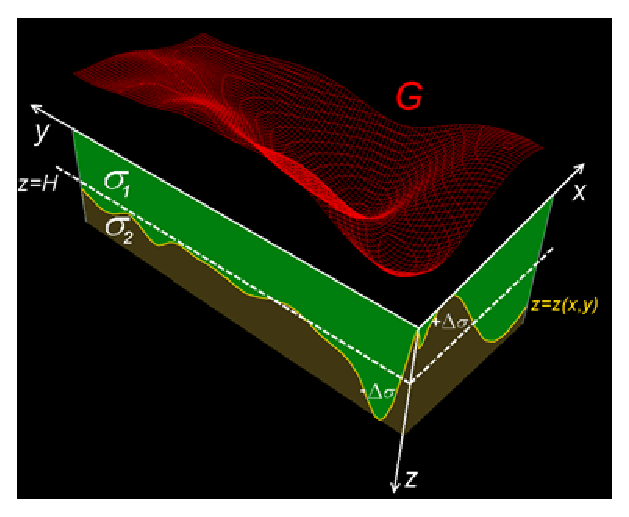
\includegraphics[height=14.0cm]{Twolaymodgrav}
	\caption{Модель двуслойной среды в задаче гравиметрии.}
	\label{fig:twolayergrav}
	\end{figure}
Запишем $\eqref{equ_grav2l}$ в виде операторного уравнения
\begin{equation}\label{equ_2lop}
	[A(u)](x,y)=-\iint_{D} \frac{1}{[(x-x')^2+(y-y')^2+u^2(x',y')]^{1/2}}dx'dy'=f(x,y),
\end{equation}
где $f(x,y)=\Delta f(x,y) 4\pi/g\Delta\sigma - A(H)$. Тогда производная оператора $A$ в точке $u^0(x,y)$ определяется формулой
$$ [A'(u^0)]h=\iint_{D} \frac{u^0(x',y')h(x',y')}{[(x-x')^2+(y-y')^2+(u^0(x',y'))^2]^{3/2}}dx'dy', $$
Уравнение (\ref{equ_2lop}) является интегральным уравнением Урысона (так как неизвестная функция $u(x,y)$ входит в ядро оператора нелинейно) I рода, следовательно, относится к классу некорректных задач.
	
После дискретизации интегрального уравнения $\eqref{equ_2lop}$ двумерным аналогом формулы прямоугольников с равномерной сеткой по каждой переменной с шагом $\Delta x$, $\Delta y$, получаем систему нелинейных уравнений относительно неизвестного вектора $u_{ji}=u(x_j,y_i)\quad (j=1,2,...,N, i=1,2,...,M)$, которая в векторно-матричном виде может быть записана следующим образом
\begin{equation}\label{equ_snle}
	A_n(u_n)=f_n,
\end{equation}
где $u_n$, $f_n$ --- векторы размерности $n=N\times M$. Дискретный аналог производной $A'(u^0)$ принимает форму
\begin{equation}\label{op_grav_disc_form}
	[A'_n(u_n^0)h_n]_{k,l}=\sum\limits_{i=1}^{M}\sum\limits_{j=1}^{N}
	\Delta x\Delta y\frac{u^0_{ji}h_{ji}}{[(x_k-x'_j)^2+(y_l-y'_i)^2+(u^0_{ji})^2]^{3/2}},
\end{equation}
где при $u_{n}^{0}=const$ матрица $A'_n(u_n^0)$ симметрична, элементы которой вычисляются по формуле $\eqref{op_grav_disc_form}$.

Рассматривается модель двухслойной среды, в которой поверхность раздела задается функцией $u(x,y)$, по формуле %\cite{AkMisSkurTre2015_1}
$$
\hat{u}(x,y)=5-3.21e^{-(x/10.13-6.62)^6-(y/9.59-2.93)^6}-
2.78e^{-(x/9.89-4.12)^6-(y/8.63-7.43)^6}$$
\begin{equation}\label{form6.5}
+3.13e^{-(x/9.89-4.82)^6-(y/8.72-4.33)^6},
\end{equation}
заданной в области $D=\{0\le x\le 100, 0\le y \le 110\}$. Была выбрана сетка с шагом $\Delta x=\Delta y=1$ (км), что приводит к размерности $n=11000$ для искомого вектора $u_n$, а также принято, что $\Delta\sigma=0.21$ (г/см$^3$), $H=5$ (км) ($z=H=5$ --- асимптотическая плоскость для $\hat{u}(x,y)$).

В результате численного эксперимента по восстановлению модельного решения $\eqref{form6.5}$ было установлено, что не только матрица $A'_n(u^0)$ имеет $n$ различных неотрицательных собственных значений, но это свойство имело место и для $A'(u_n^k)$ на каждой $k$-итерации. Тем самым выполнены условия, при которых получены результаты в данной главе по сходимости и оценке погрешности процессов $\eqref{equ_rmn}$, $\eqref{equ_alphaproc}$ для немонотонного оператора $A$ с положительным спектром. 

При анализе числа обусловленности $\mu(A'_n(u_n^k))$ было установлено, что эта величина для всех четырех процессов принимала значения $\mu(A'_n(u_n^k))\approx 4.6 * 10^{8}$ для немодифицированного варианта и $\mu(A'_n(u_n^0))\approx 1.5 * 10^{4}$ для модифицированных методов. Выход из процесса итераций каждого из методов осуществлялся по правилу
\begin{equation}\label{cond6.6}
\frac{\|\hat{u}_n-\tilde{u}_n\|_{R^n}}{\|\tilde{u}_n\|_{R^n}}\le 10^{-2},
\end{equation}
где $\hat{u}_n$ --- точное решение системы уравнений $\eqref{equ_snle}$, а $\tilde{u}_n$ --- восстановленное каждым из четырех итерационных методов. Таким образом, точность численного решения, полученного процессами $\eqref{equ_rmn}$, $\eqref{equ_alphaproc}$ и их модифицированными аналогами, гарантированно не превышала $\varepsilon=10^{-2}$.

В таблице $\ref{Table_gravy}$ представлены результаты расчетов при значениях параметров $\bar\alpha=\alpha=10^{-3}$, $\gamma=1$, где
\begin{equation}\label{form6.7}
\Delta=\frac{\|A_n(\tilde{u}_n)+\alpha(\tilde{u}_n-u^0)-f_n\|_{R^n}}{\|f_n\|_{R^n}},
\end{equation}
относительная регуляризованная невязка для восстановленного решения, $N_\varepsilon$ --- число итераций в процессе для достижения точности, определяемой неравенством $\eqref{cond6.6}$, $T$ --- время реализации метода. В позициях для $\Delta$, $N_\varepsilon$, $T$ верхняя строка соответствует основным процессам, а нижняя --- их модифицированным вариантам.
\begin{table}[H]
	\centering
	\renewcommand{\arraystretch}{1.5}
	\caption{Эксперименты для обратной задачи гравиметрии}
	\label{Table_gravy}
	\begin{tabular}{|p{0.2\textwidth}|p{0.1\textwidth}|p{0.1\textwidth}|p{0.1\textwidth}|p{0.1\textwidth}|}
		\hline
		\rule{0cm}{0.5cm}
		\textbf{Методы} & \textbf{ММО} & \textbf{МНС} & \textbf{ММН} & \textbf{РМН} \\ \hline
		\rule{0cm}{0.5cm}
		{$\Delta$} & 0.0048 & 0.0020 & 0.0024 & 0.0023	 \\ \cline{2-5} 
		\rule{0cm}{0.5cm}
		&  0.0094   & 0.0019    &  0.0019   &  0.0021   \\ \hline
		\rule{0cm}{0.5cm}
		{$N_\varepsilon$} & 17  &  21   &   20  &  16    \\ \cline{2-5}
		\rule{0cm}{0.5cm}
		&  22   &   23  &  23   &  16   \\ \hline
		\rule{0cm}{0.5cm}
		{$T$ (сек)}    &  30   &  11   &  14  & 27    \\ \cline{2-5}
		\rule{0cm}{0.5cm}
		& 35   & 12    &  15   &   26  \\ \hline
	\end{tabular}
\end{table}

{\bfseries 2.4.2. Решение структурной обратной задачи магнитометрии}
 
Уравнение магнитометрии при тех же предположениях, что и в задаче гравиметрии для двухслойной среды, имеет вид
\begin{equation}\label{equ_magn}\begin{aligned}
\Delta J  \bigg\{&\iint_{D} \frac{H}{[(x-x')^2+(y-y')^2+H^2]^{3/2}}dx'dy' \\
- &\iint_{D} \frac{u(x',y')}{[(x-x')^2+(y-y')^2+u^2(x',y')]^{3/2}}dx'dy' \bigg\}=\Delta G(x,y),
\end{aligned} \end{equation}
где $\Delta J$ --- усредненный скачок $z$-компоненты вектора намагниченности, $z=H$ --- асимптотическая плоскость, $u(x,y)$ --- функция, описывающая аномальное поле, $z=u(x,y)$ --- искомая функция, описывающая поверхность раздела сред с различными свойствами намагниченности (рис.~\ref{fig:twolayermag}). 
\begin{figure}[H]
	\centering
	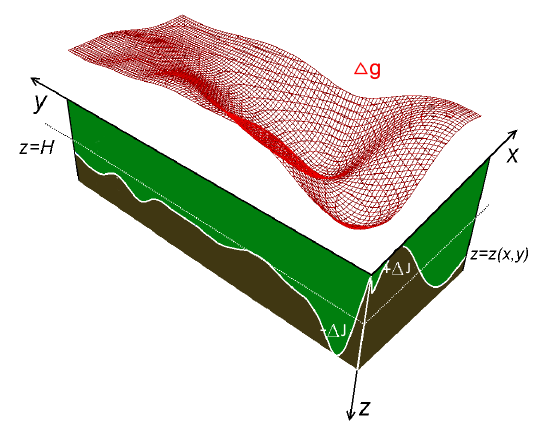
\includegraphics[height=14.0cm]{Twolaymodmag}
	\caption{Модель двуслойной среды в задаче магнитометрии.}
	\label{fig:twolayermag}
\end{figure}
Уравнение $\eqref{equ_magn}$ можно переписать в форме
\begin{equation}\label{equ_magn_op}
[D(u)](x,y)= \iint_{D} \frac{u(x',y')}{[(x-x')^2+(y-y')^2+u^2(x',y')]^{3/2}}dx'dy'=F(x,y),
\end{equation}
где $F(x,y)=D(H)-\Delta G(x,y)/\Delta J$, тогда производная оператора $D$ в точке $u^0(x,y)$ определится формулой
$$ [A'(u^0)]h=\iint_{D} \frac{(x-x')^2+(y-y')^2-2(u^0(x',y'))^2}{[(x-x')^2+(y-y')^2+(u^0(x',y'))^2]^{5/2}}h(x',y')dx'dy'. $$

После дискретной аппроксимации, подобно задаче гравиметрии уравнения $\eqref{equ_magn_op}$, приходим к системе нелинейных уравнений
\begin{equation}\label{equ_snle_mag}
D_n(u_n)=F_n
\end{equation}
относительно вектора $u_n \quad (n=N\times M)$ с компонентами $u_{ij}\quad (i=1,2,...,N, j=1,2,...,M)$, при этом компоненты производной оператора $D_n$ в точке $u_{n}^{0}$ вычисляются по формуле
\begin{equation}\label{deriv_op_mag}
[D'_n(u_{n}^{0})h_n]_{k,l}=\sum\limits_{i=1}^{N}\sum\limits_{j=1}^{M}
\Delta x\Delta y\frac{(x_k-x'_j)^2+(y_l-y'_i)^2-2(u_{ji}^0)^2}{[(x_k-x'_j)^2+(y_l-y'_i)^2+(u_{ji}^0)^2]^{5/2}}h_{ji}, 
\end{equation}
причем при $u_{n}^{0}=\{u^0(x'_j, y'_i), 1\le j\le M, 1\le i\le N\}=const$, $D'_n(u_n^0)$ --- симметричная матрица.

Модельное решение уравнения $\eqref{equ_snle_mag}$, определяющее поверхность раздела сред, задается формулой \cite{AkMisDer2014}
\begin{equation}\label{form6.11}
\hat{u}(x,y)=5-2e^{-(x/10-3.5)^6-(y/10-2.5)^6}-
3^{-(x/10-5.5)^6-(y/10-4.5)^6},
\end{equation}
на области $D=\{0\le x \le 100, 0\le y\le 100\}$. Сетка строилась с шагом $\Delta x=\Delta y = 1$ (км), что влечет размерность $n=10000$ для искомого вектора $u_n$.

Для $\Delta J=0.4$  был выполнен численный эксперимент по восстановлению модельного решения задачи $\eqref{equ_magn_op}$ процессами $\eqref{equ_rmn}$, $\eqref{equ_alphaproc}$ при $\bar\alpha=0.01$, $\alpha = 0.0001$, $\beta=1$, а также их модифицированными аналогами, когда производная $D'(u^k)$ вычисляется в фиксированной точке $u_n^0=H=5$ (км). Число обусловленности $\mu(D'_n(u_n^0))=1.8\cdot 10^7$. После вычисления спектра матрицы $D'_n(u_n^k)$ выяснилось, что она имеет различные неотрицательные собственные значения, что на основании теорем сходимости главы 2, при подходящем выборе параметра $\beta$ и начальном приближении $u_n^0$, гарантирует сходимость итерационных схем и двухэтапного метода. Окончание итерационных процессов выполнялось по правилу $\eqref{cond6.6}$.

Результаты численных расчетов для задачи $\eqref{equ_snle_mag}$ по восстановлению модельного решения $\eqref{form6.11}$ представлены в таблице $\ref{Table_magne}$. Как и в таблице $\ref{Table_gravy}$, здесь $\Delta$ --- относительная норма невязки $\eqref{form6.7}$ для восстановленного решения, $N_\varepsilon$ --- число итераций для достижения точности $\eqref{cond6.6}$, $T$ --- машинное время при реализации процесса, верхние строки для каждого параметра соответствуют данным для основных (немодифицированных) процессов $\eqref{equ_rmn}$, $\eqref{equ_alphaproc}$, нижние строки --- для модифицированных вариантов $\eqref{equ_rmn}$, $\eqref{equ_alphaproc}$.
\begin{table}[H]
	\centering
%	\renewcommand{\arraystretch}{1.5}
	\caption{Эксперименты для обратной задачи магнитометрии}
	\label{Table_magne}
	\begin{tabular}{|p{0.2\textwidth}|p{0.1\textwidth}|p{0.1\textwidth}|p{0.1\textwidth}|p{0.1\textwidth}|}
		\hline
		\rule{0cm}{0.5cm}
		\textbf{Методы} & \textbf{ММО} & \textbf{МНС} & \textbf{ММН} & \textbf{РМН} \\ \hline
		\rule{0cm}{0.5cm}
		{$\Delta$} & 0.0636 & 0.0699 & 0.0802 & 0.0368	 \\ \cline{2-5} 
		\rule{0cm}{0.5cm}
		&  0.0569   & 0.0575    &  0.0595   &  0.0369   \\ \hline
		\rule{0cm}{0.5cm}
		{$N_\varepsilon$} & 4  &  4   &   4  &  5    \\ \cline{2-5}
		\rule{0cm}{0.5cm}
		&  4   &   4  &  4   &  5   \\ \hline
		\rule{0cm}{0.5cm}
		{$T$ (сек)}    &  7   &  6   &  6  & 22    \\ \cline{2-5}
		\rule{0cm}{0.5cm}
		& 5    & 3    &  3   &   3  \\ \hline
	\end{tabular}
\end{table}

{\bfseries\large Вывод.} Анализируя результаты численного эксперимента для задач гравиметрии и магнитометрии, можно отметить, что для достижения одной и той же точности приближенного решения в соответствии с правилом $\eqref{cond6.6}$, число итераций для модифицированных методов, как правило, больше, чем немодифицированных процессов $\eqref{equ_rmn}$, $\eqref{equ_alphaproc}$. Однако затраты машинного времени при реализации модифицированных процессов, за исключением ММО, существенно меньше. Поэтому можно сделать вывод, что модифицированные МНС, ММН и РМН более экономичны и, следовательно, более предпочтительны для некоторых классов нелинейных задач большой размерности. Более затратная по времени реализация ММО, по сравнению с МНС и ММН, связана прежде всего с тем, что в коэффициенте $\beta_{-1}(u^k)$ необходимо вычислять не только скалярные произведения, но и обращать на каждом шаге оператор $B_k=A'(u^k)+\alpha I$. Следует сказать, что для уравнения $\eqref{equ1}$ ММО обычно не используется. Его применение целесообразно для эквивалентного уравнения $A'(u)^*(A(u)-f)=0$, для которого ММО преобразуется к виду, где операция обращения отсутствует [\cite{VasEre2009},	c.~57, формула 5.8]. Заметим также, что в методе ММО и РМН вычисление элемента вида $W=(A'(u^k)+\alpha I)^{-1}V$ заменялось приближенным решением системы $(A'(u^k)+\alpha I)W=V$ с помощью метода минимальных невязок, т.е. в этом случае фактически реализуется гибридная схема градиентно--ньютоновского типа. 

Как можно видеть из таблицы $\ref{Table_magne}$, также тенденция по затратам машинного времени для модифицированных вариантов процессов $\eqref{equ_rmn}$, $\eqref{equ_alphaproc}$ (включая ММО) также сохраняется и для обратной задачи магнитометрии. 


%\section{Выводы ко второй главе}